\subsection{The scale and timing of low-credibility AI disclosure}

We begin with a descriptive analysis. Figure~\ref{fig:mismatch_surge} shows that low-credibility AI disclosure becomes common quickly in the post-2022 period. The number of AI-talking firm-years flagged as PatentMismatch rises sharply after 2022, and the mismatch share among AI-talking firm-years reaches 41.48\% in 2024 and 42.12\% in 2025. The recent expansion of AI language in annual filings is not simply a broad increase in AI-related discussion; it is also associated with a rapid increase in the subset of firm-years in which disclosure composition appears difficult to reconcile with contemporaneous AI patenting.

\begin{figure}[p]
\centering
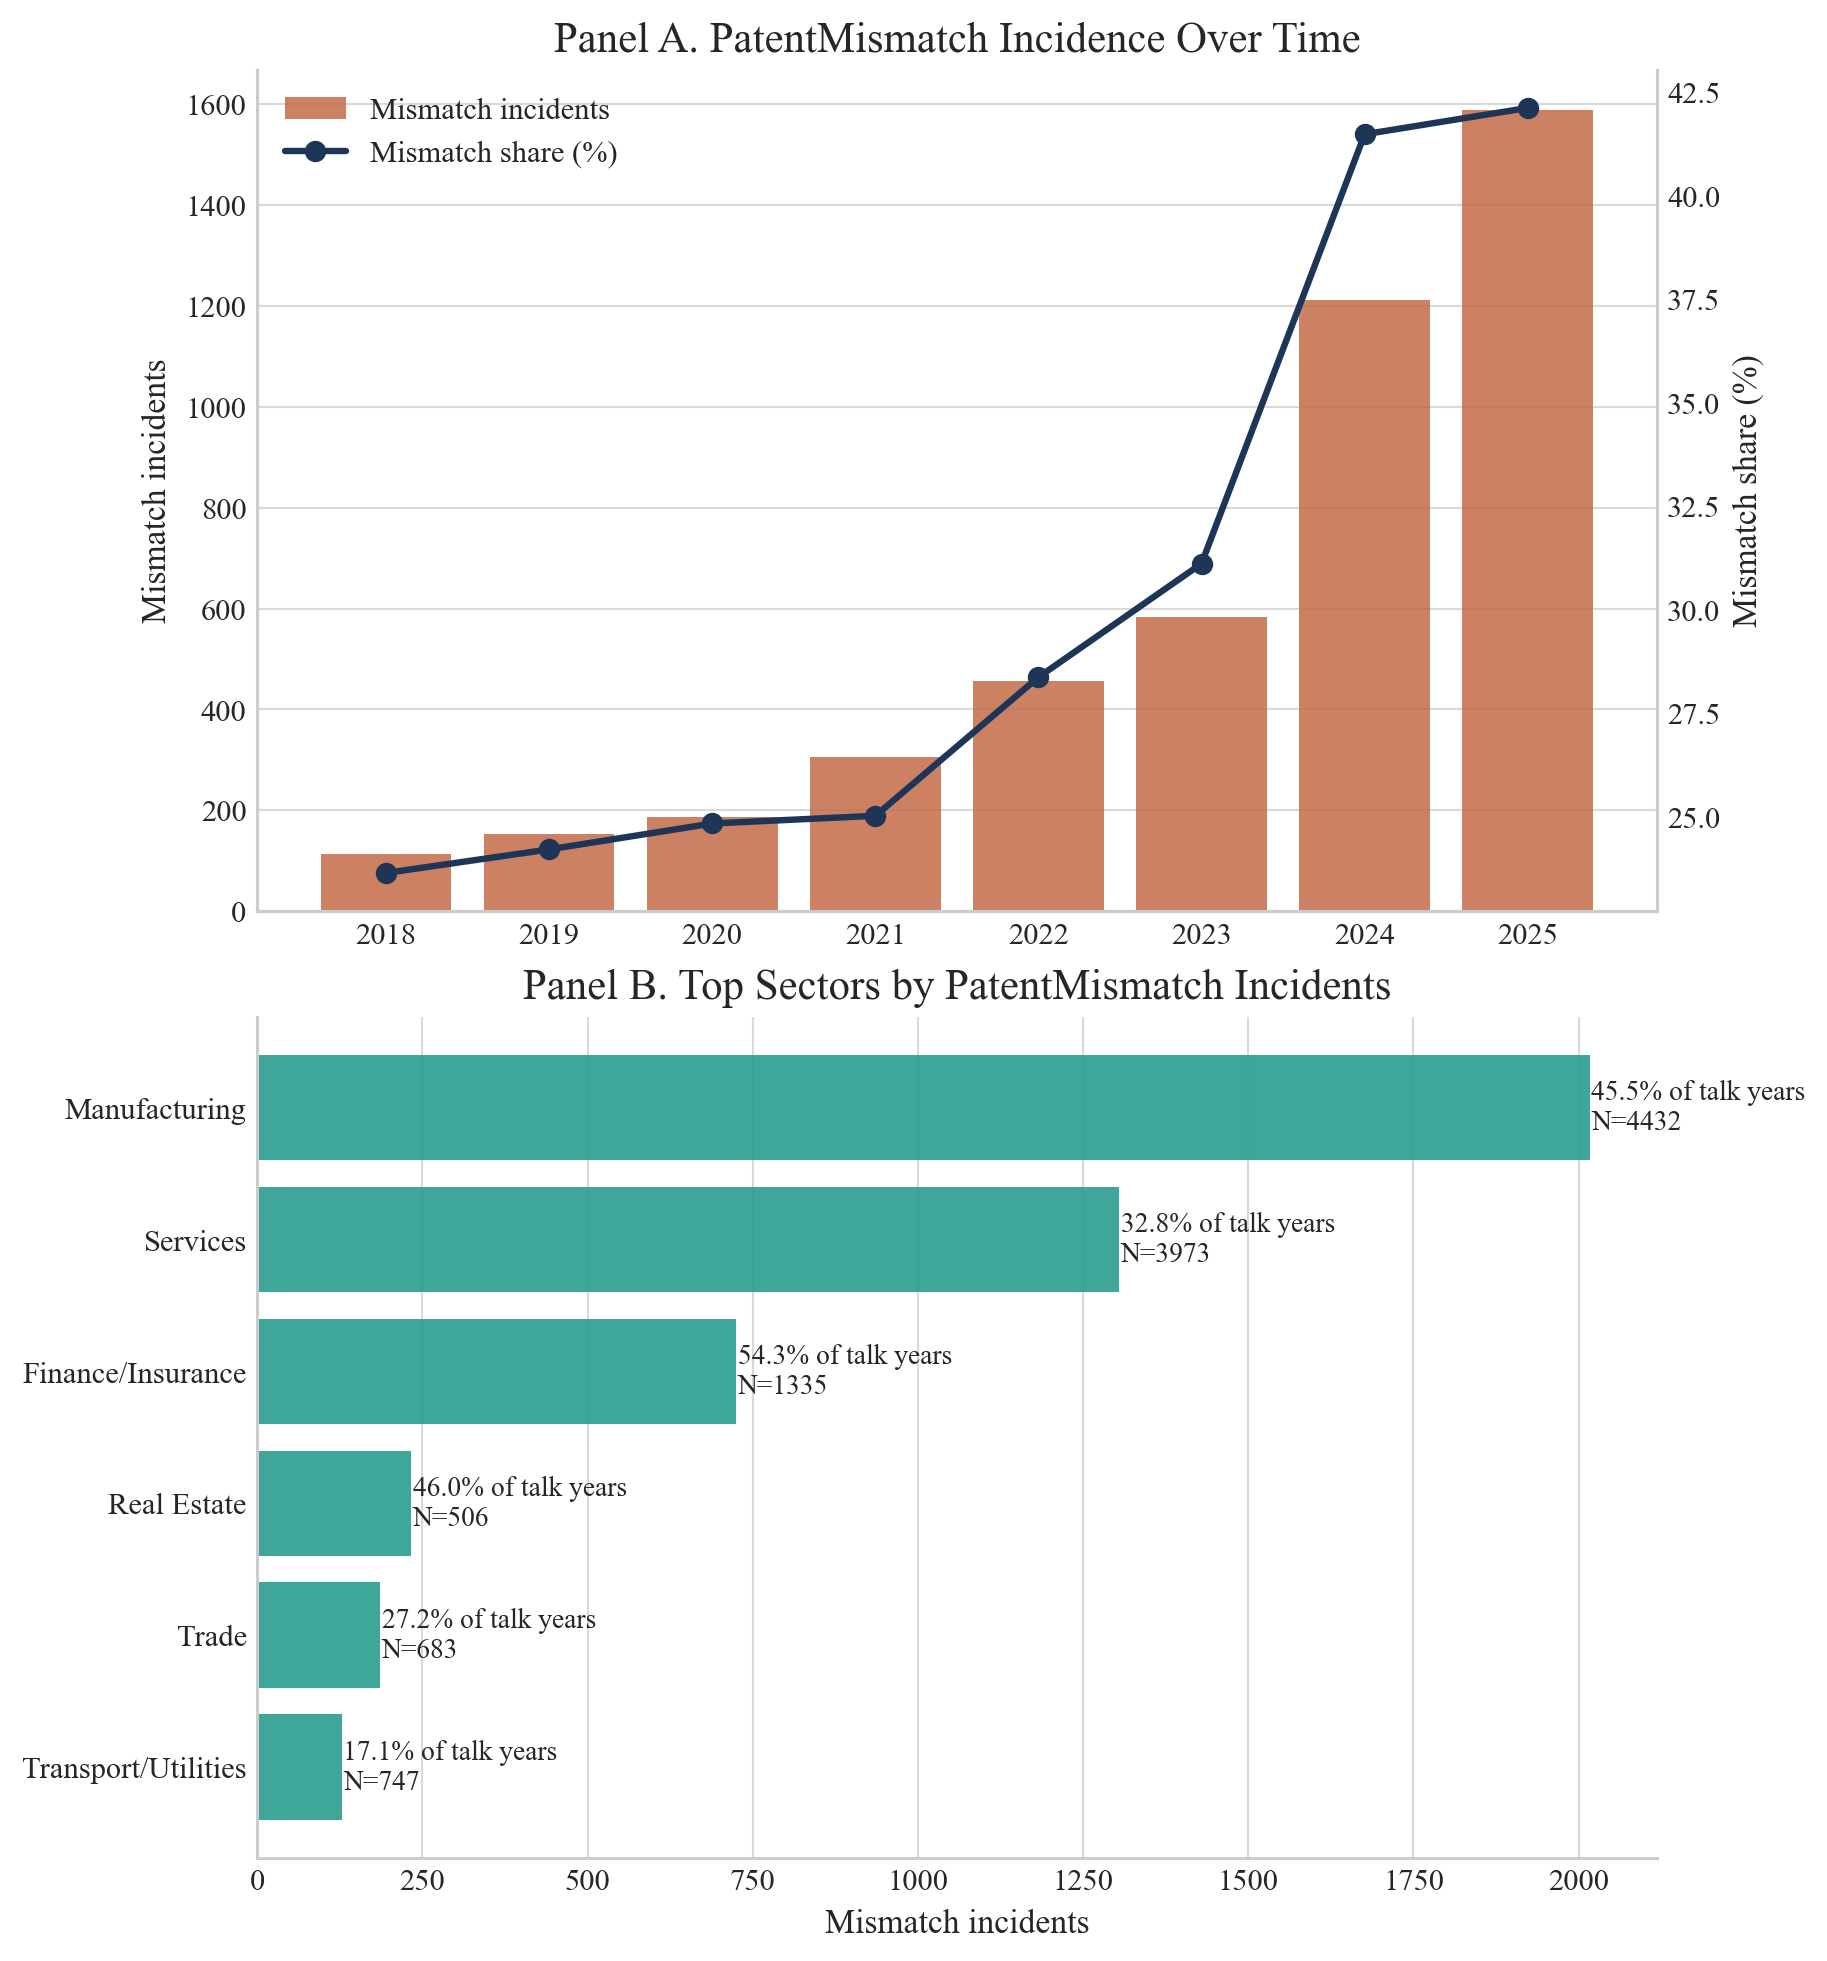
\includegraphics[width=\textwidth]{figures/figure1.png}
\caption{PatentMismatch surge through 2025}
\label{fig:mismatch_surge}
\end{figure}

Table~\ref{tab:summary_stats} describes the expanded ever-speaker annual panel and the linked filing-event sample used in the current paper. The panel contains 50,840 firm-year observations across 5,084 firms, of which 13,777 are AI-talking firm-years, and the classified corpus contains 147,879 AI-related sentences. AI-related disclosure remains highly skewed, and AI patenting remains sparse in the cross section, even within the ever-speaker universe. Those distributional features are important for interpretation. We are studying a setting in which narrative expansion has become widespread, while observable implementation remains concentrated in a much smaller subset of firms.

\tablepdf
{Summary statistics}
{tab:summary_stats}
{This table presents summary statistics for the variables used in the analysis. It reports the mean, standard deviation, selected percentiles, and the number of observations for the expanded ever-speaker annual panel.}
{tables/table1.png}

Figures~\ref{fig:descriptive_background} and \ref{fig:patent_background} provide a more general descriptive backdrop. Figure~\ref{fig:descriptive_background} traces the increase in the volume of AI-related disclosure and the evolution of disclosure composition over time. Figure~\ref{fig:patent_background} shows that AI patenting also increases over the sample, but much more gradually and at a lower base. With Figure~\ref{fig:mismatch_surge}, these descriptive patterns clarify why the mismatch construct is economically interesting. The growth in AI talk appears to outpace the growth in visible technological realization for a substantial subset of firms.

\begin{figure}[p]
\centering
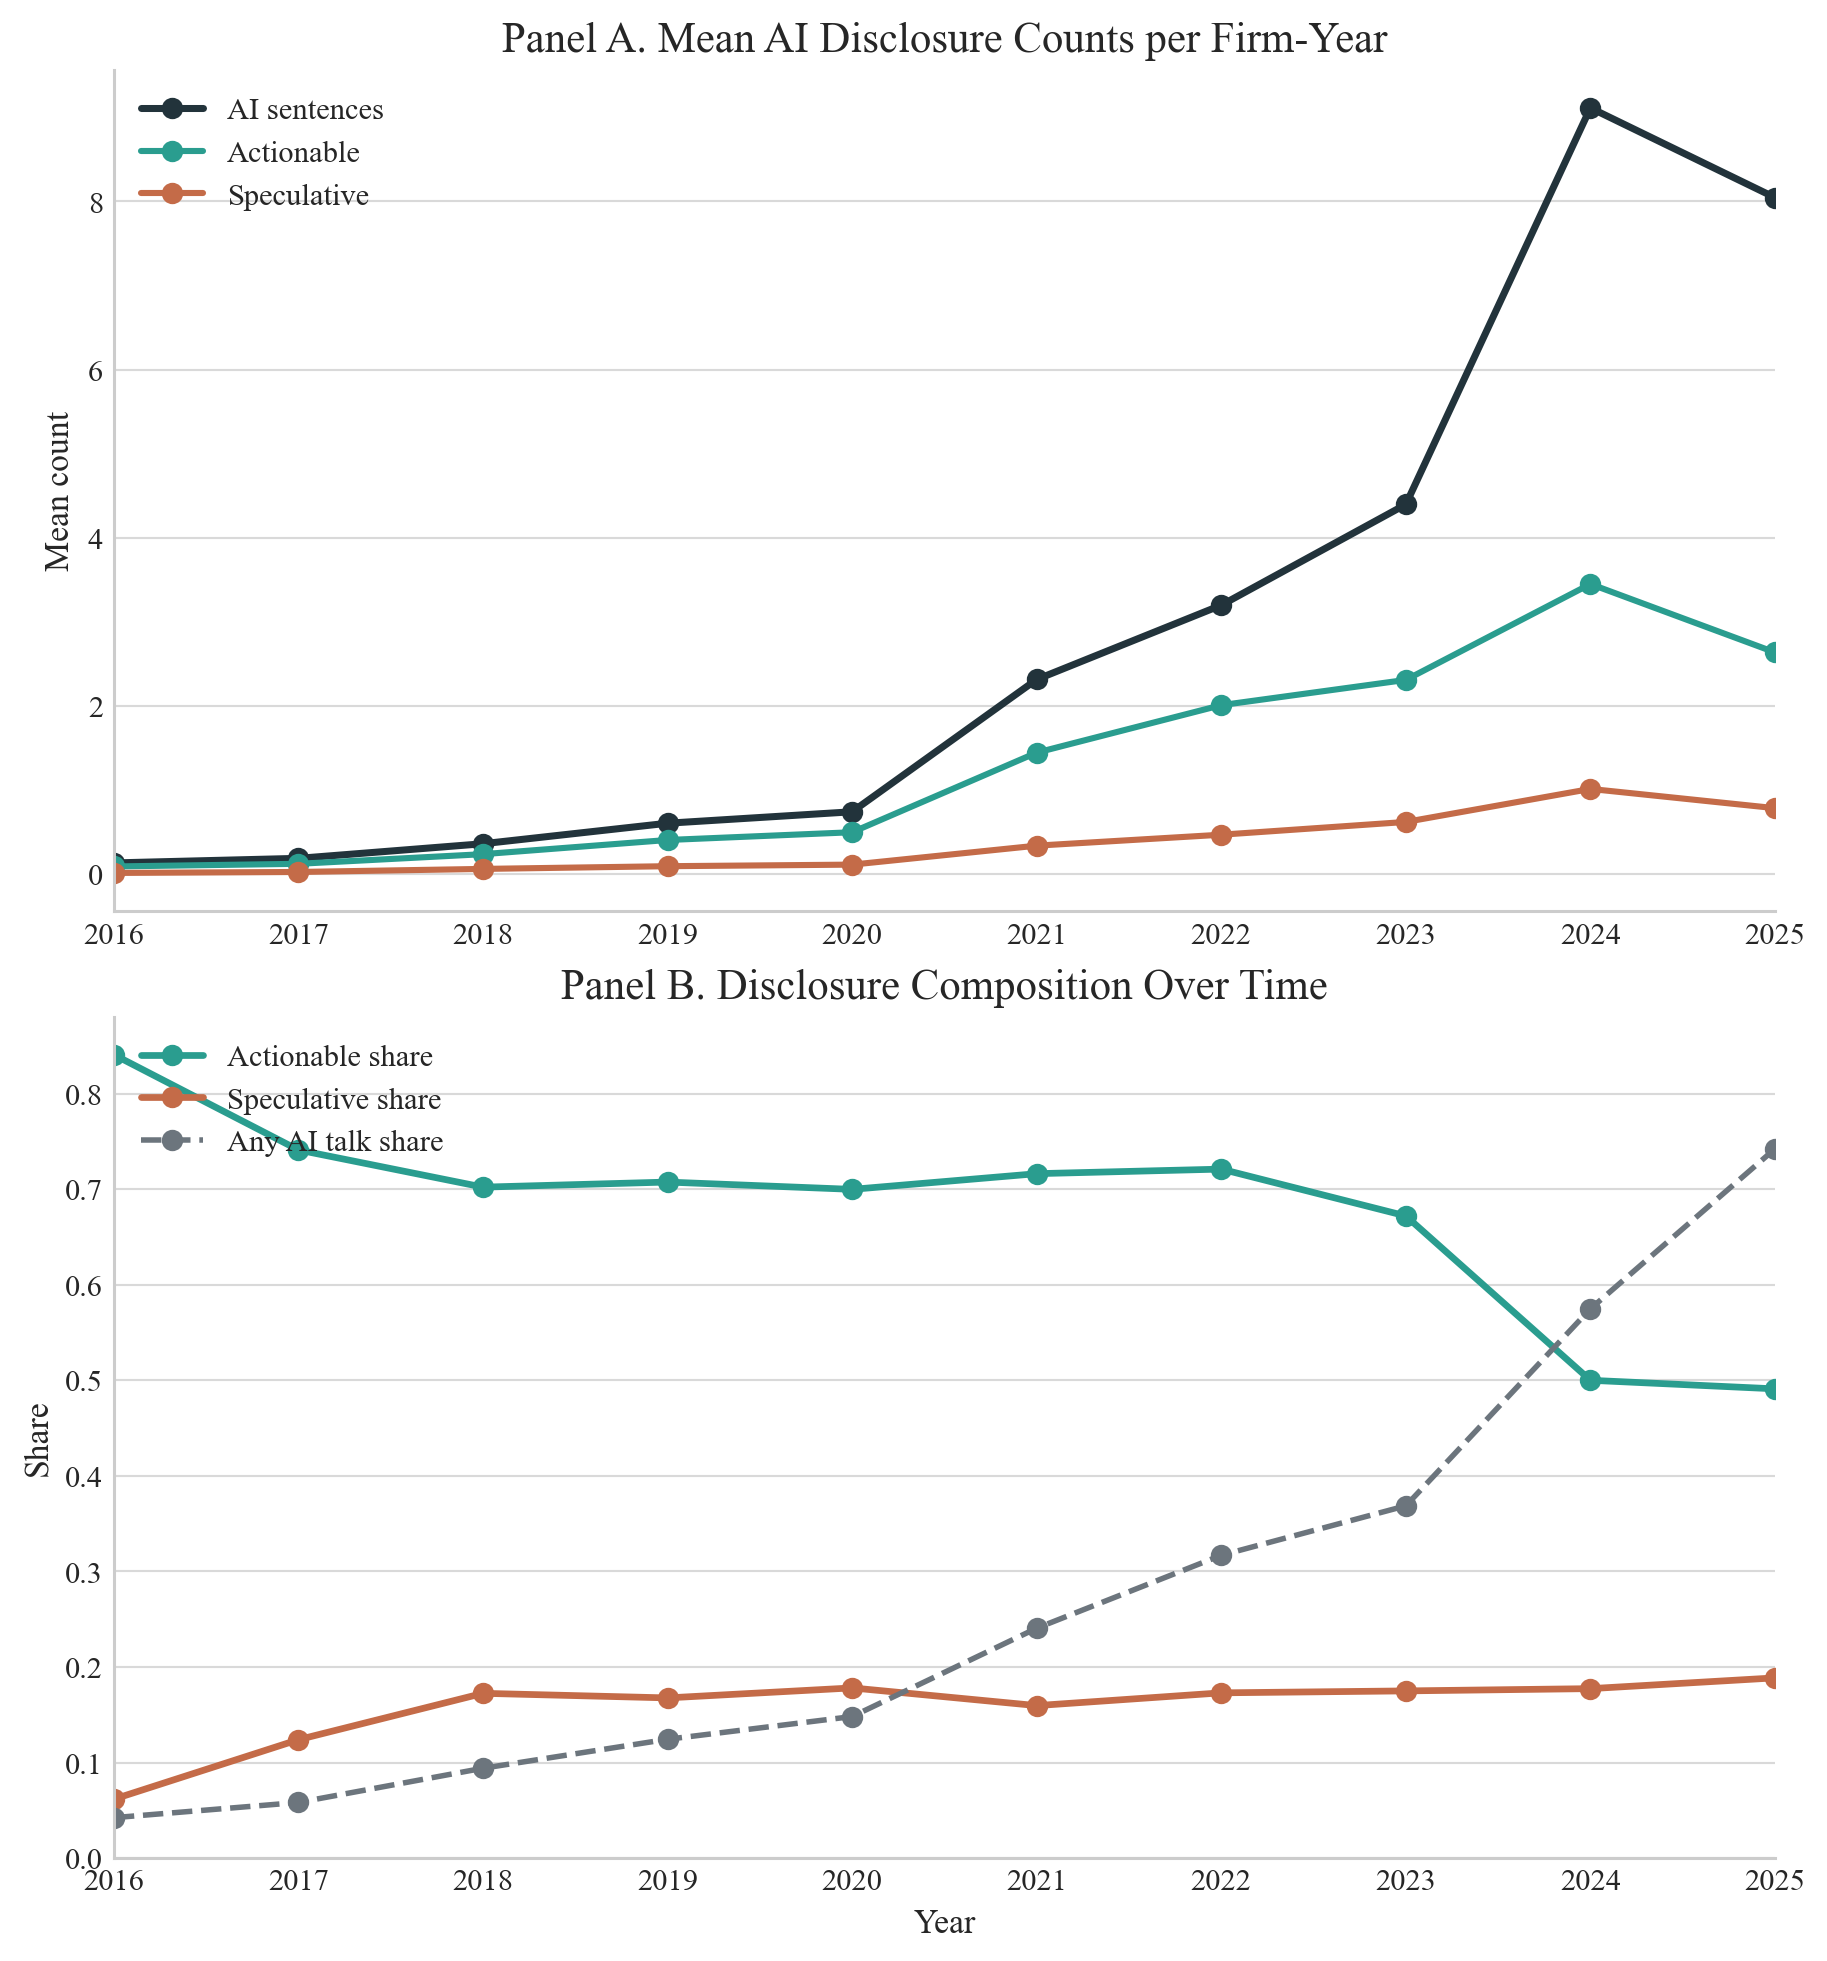
\includegraphics[width=\textwidth]{figures/figure2.png}
\caption{Disclosure volume and composition over time}
\label{fig:descriptive_background}
\end{figure}

\begin{figure}[p]
\centering
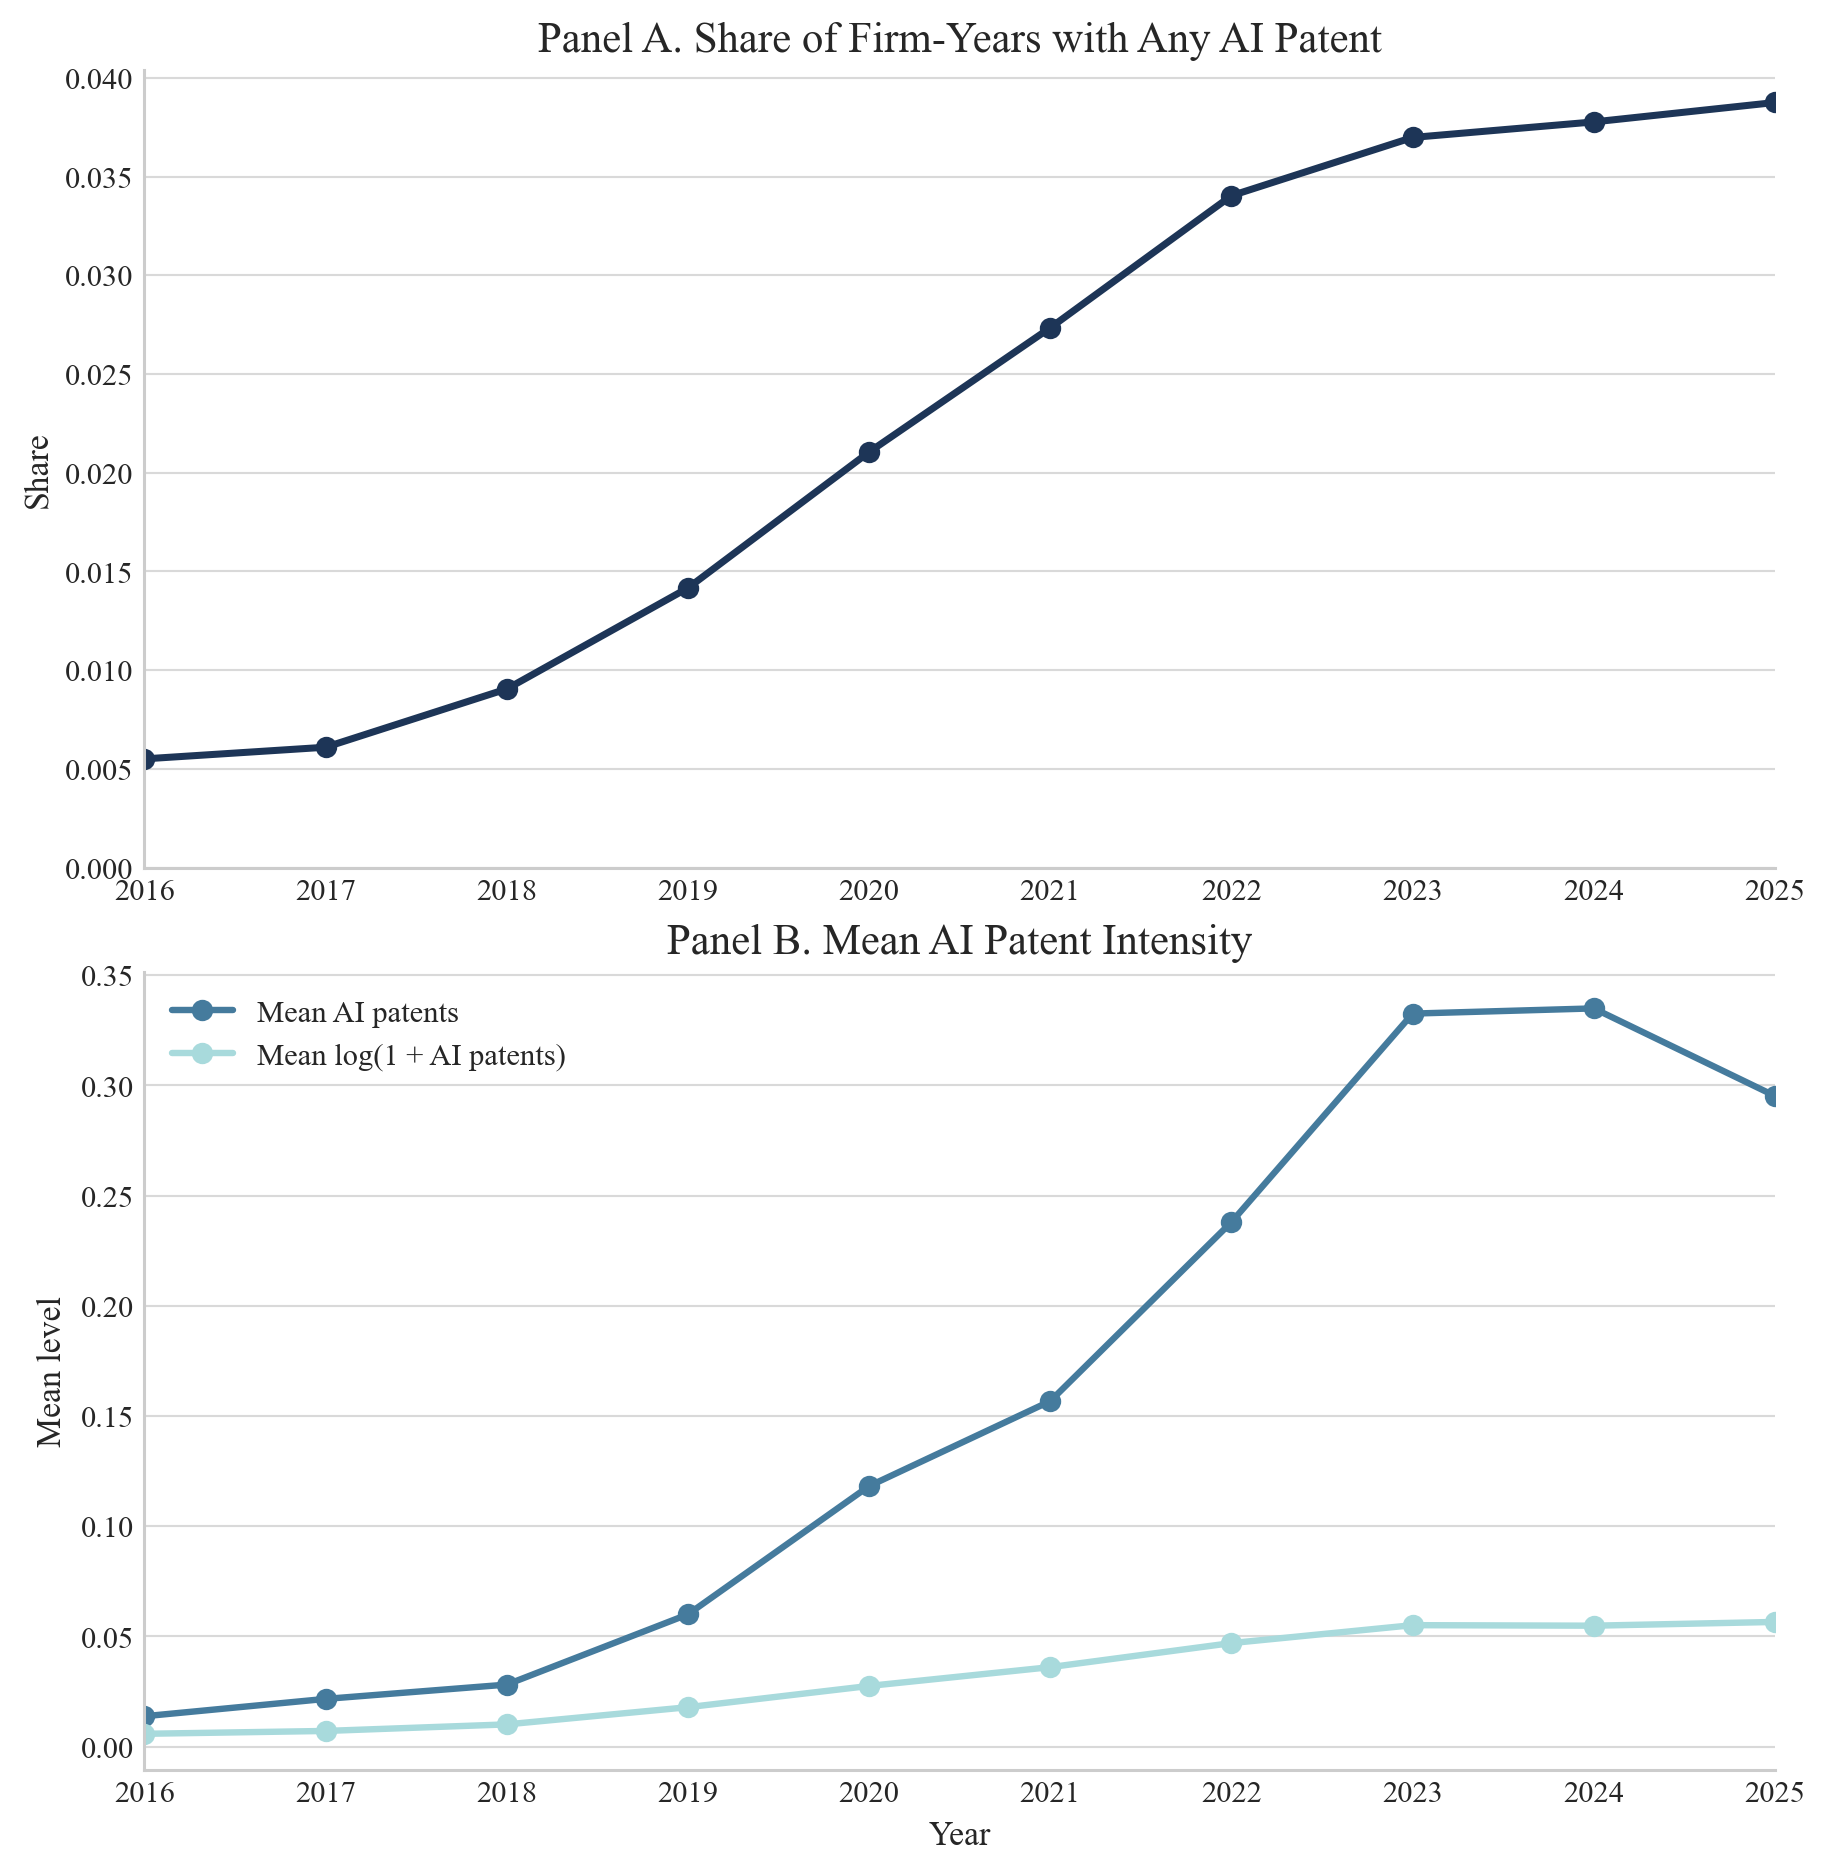
\includegraphics[width=\textwidth]{figures/figure3.png}
\caption{AI patent coverage over time}
\label{fig:patent_background}
\end{figure}

\subsection{Markets do not fully sort low-credibility AI disclosure at the filing date}

The first market-based question is whether investors distinguish low-credibility AI disclosure immediately when the annual 10-K is released. Table~\ref{tab:filing_date_car} suggests that they do not, at least not in a clean or robust way. In the narrow filing window, the difference in market-adjusted abnormal returns between mismatch and non-mismatch AI filers is small and statistically insignificant. The mismatch-minus-non-mismatch mean difference in CAR[$-1,+1$] is 0.115 percentage points with a p-value of 0.678, and the corresponding filing-level regression coefficient on PatentMismatch is 0.0015 with a p-value of 0.702. The same conclusion holds in the slightly wider CAR[$-2,+2$] window. The filing date does not appear to cleanly separate mismatch from non-mismatch firms in return space.

\tablepdf
{Filing-date abnormal returns around annual 10-K releases}
{tab:filing_date_car}
{This table reports market-adjusted filing-date cumulative abnormal returns around annual 10-K releases. Panel A reports mean CARs by PatentMismatch status and the mismatch-minus-non-mismatch difference. Panel B reports filing-level regressions of CAR on PatentMismatch, the AS ratio, and AI Focus with lagged controls, industry fixed effects, filing-year fixed effects, and standard errors clustered by firm. Statistical significance at the 1\%, 5\%, and 10\% levels is indicated by ***, **, and *, respectively. A CAR[$-5,+5$] column is not included in this first run because the current daily event-return scaffold starts at event day $-2$.}
{tables/table2.png}

\subsection{The sharper pricing pattern emerges after the filing}

If the filing date does not provide a clean correction, the next question is whether the pricing response unfolds more gradually. Figure~\ref{fig:post_filing_drift} and Table~\ref{tab:portfolio_alpha} suggest that it does. The event-time figure shows that the return paths separate after the filing window rather than at it, which is more consistent with slower incorporation than with an immediate market response. The sharper return-based pattern appears in the calendar-time portfolio tests. A long--short strategy that buys firms with more credible AI disclosure and shorts mismatch firms earns its strongest return over the subsequent quarter in the equal-weight specification. The equal-weight 3-month portfolio delivers a market alpha of 0.926 percentage points per month (p = 0.047), or approximately 11.2\% annualized. By contrast, the value-weighted 3-month alpha is essentially zero. The pattern weakens at the 12-month horizon. That combination of results suggests that the post-filing effect is concentrated in shorter horizons and outside the largest firms, which is consistent with a slower correction in harder-to-value companies rather than a broad market-wide repricing.

\begin{figure}[p]
\centering
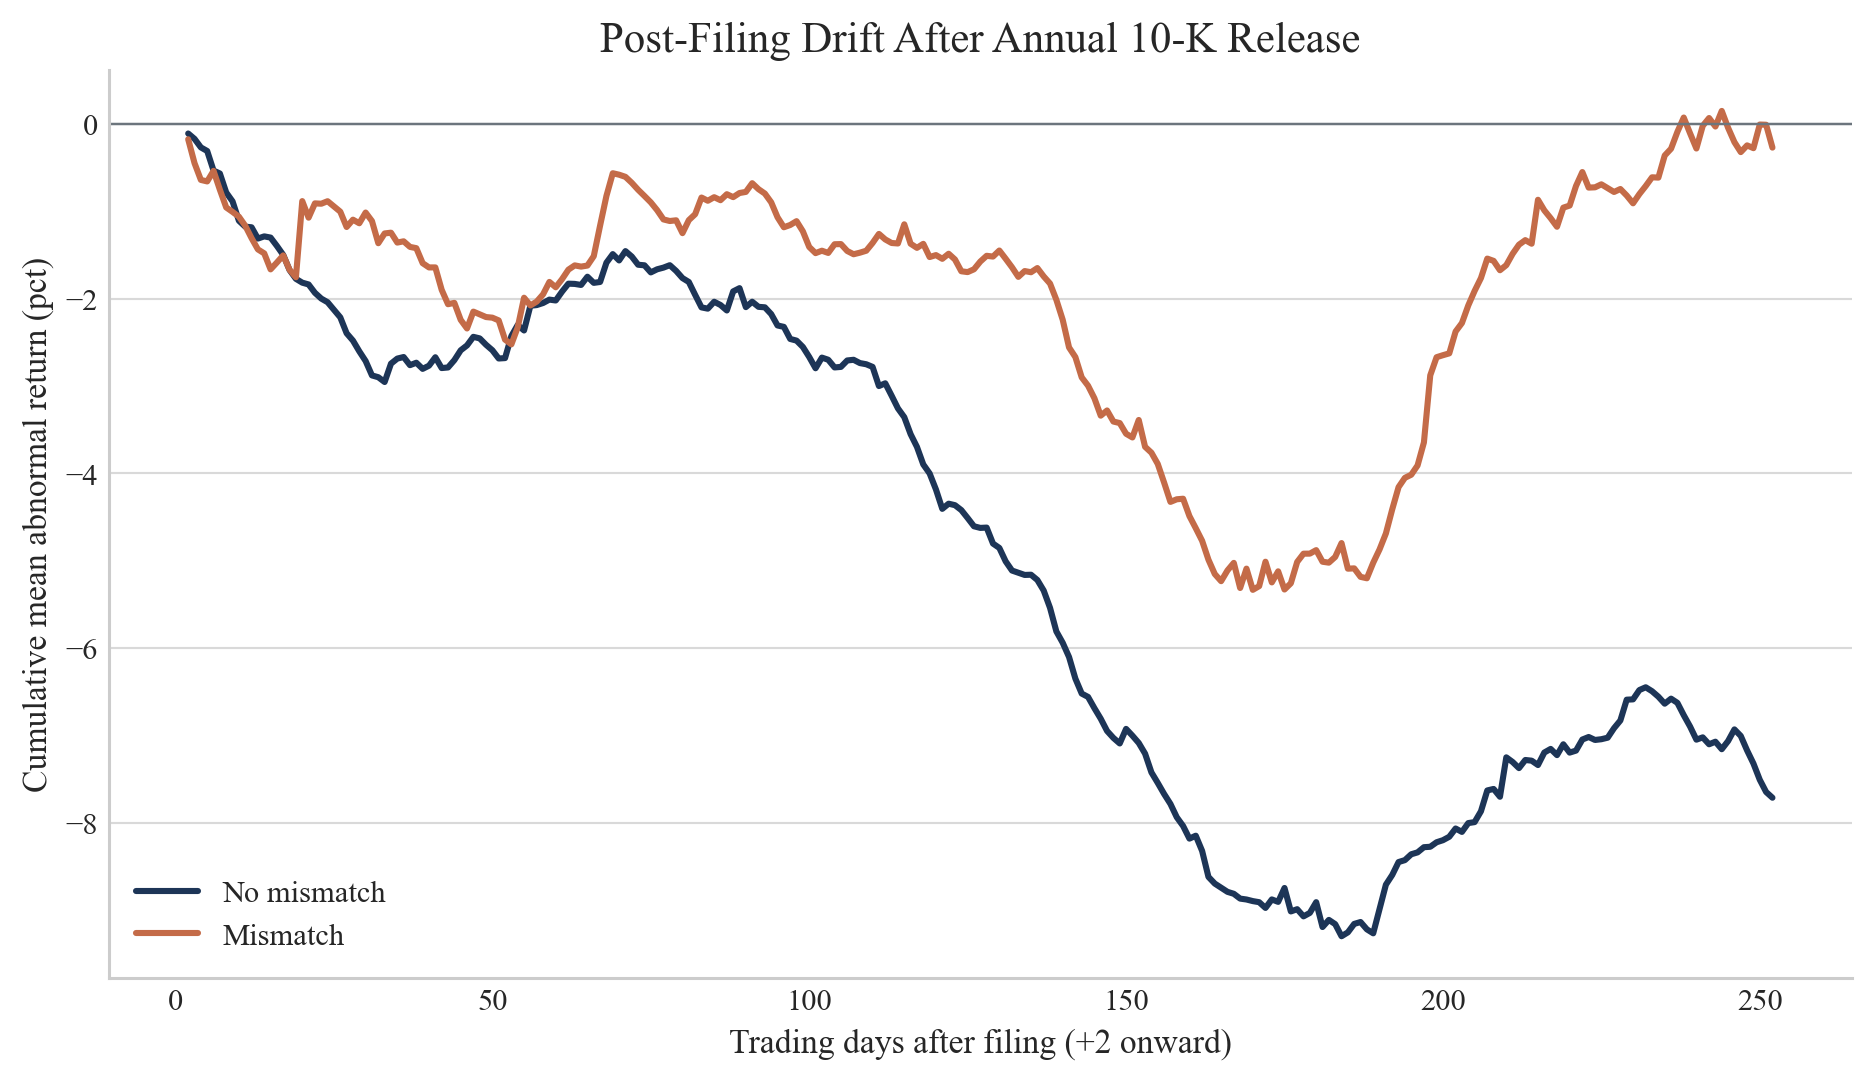
\includegraphics[width=\textwidth]{figures/figure4.png}
\caption{Post-filing drift after annual 10-K release}
\label{fig:post_filing_drift}
\end{figure}

\tablepdf
{Calendar-time long--short portfolio returns after filing signals}
{tab:portfolio_alpha}
{This table reports calendar-time long--short portfolio returns formed after AI-related annual filing signals. Each month, the long leg holds non-mismatch AI filers and the short leg holds mismatch AI filers that filed within the prior 1, 3, 6, or 12 months. Panel A reports equal-weight portfolios and Panel B reports value-weight portfolios using lagged market capitalization. Market alpha is the intercept from a regression of the long--short monthly return on the CRSP value-weighted market return. Panel C splits the three-month portfolio on whether the underlying filing signal occurred before or after the ChatGPT regime shift.}
{tables/table3.png}

\subsection{Cross-sectional valuation and financing consequences}

Valuation and financing tests ask whether the same disclosure-credibility construct appears in broader annual market outcomes. Table~\ref{tab:valuation_financing_nonbig} reports the cleaner non-big-firm specifications, where the current effects are strongest. The valuation results are positive and marginally significant: PatentMismatch is associated with higher log market-capitalization-to-assets and a higher log Tobin's-$Q$ proxy, with coefficients of 0.0619 (p = 0.065) and 0.0627 (p = 0.062), respectively. The financing side is much weaker. Neither next-year share growth nor the indicator for substantial issuance shows a meaningful relation to PatentMismatch in this sample. This implies that the more credible cross-sectional consequence in the current data is valuation, and that this valuation pattern is most visible outside the largest firms.

\tablepdf
{Financing and valuation consequences in non-big firms}
{tab:valuation_financing_nonbig}
{This table reports valuation and financing consequences associated with disclosure credibility in the non-big subsample. Panel A uses log market-capitalization-to-assets, a log Tobin's-$Q$ proxy equal to log(1 + market-capitalization-to-assets + leverage), and the next-year change in that log $Q$ proxy. Panel B uses next-year change in CRSP shares outstanding and an indicator for share growth above 5\%. The key regressors are PatentMismatch, the AS ratio, and AI Focus. All specifications absorb firm and year fixed effects and use firm-clustered standard errors.}
{tables/table4.png}

\subsection{Real consequences and validation of the disclosure construct}

Market-based evidence suggests that low-credibility AI disclosure is not fully sorted out at the filing date and that slower correction is strongest outside the largest firms. The next question is whether the same disclosure-credibility construct is informative for subsequent real outcomes. Table~\ref{tab:real_effects} reports that PatentMismatch is associated with materially lower future ROA at the two-year horizon, with a coefficient of $-0.0582$ (p = 0.004), while the AS ratio is negatively related to future sales growth at the one-year horizon, with a coefficient of $-0.0826$ (p = 0.009), suggesting that the disclosure-credibility construct has a forward link to operating and innovation-related outcomes beyond the immediate market-response block.

\tablepdf
{Real effects beyond immediate market outcomes}
{tab:real_effects}
{This table reports forward operating and innovation-related outcomes associated with disclosure credibility. The dependent variables include future ROA and future sales growth at annual horizons. The key regressors are PatentMismatch, the AS ratio, and AI Focus. All specifications use the annual ever-speaker panel and absorb firm and year fixed effects with firm-clustered standard errors.}
{tables/table5.png}

The next question is whether the disclosure composition itself still behaves as expected once  beyond broad AI-talk counts. Table~\ref{tab:composition_timing} reports that actionable disclosure remains positively associated with later AI-related patenting, with coefficients of 0.042 in both $t$ and $t+1$, and 0.039 in $t+2$, which are all strongly significant. Speculative-only disclosure behaves differently. Its coefficient is negative at $t$ ($-0.044$, p $< 0.05$) and effectively disappears by $t+1$. The market and mismatch analysis therefore rest on a disclosure measure that continues to separate more implementation-linked AI language from weaker, more rhetorical AI language.

\tablepdf
{Disclosure composition and AI patent timing}
{tab:composition_timing}
{This table reports annual panel regressions linking disclosure composition to AI patent timing. Panel A uses the actionable-disclosure indicator and Panel B uses the speculative-only indicator. The dependent variable is $\log(1+\text{AI patents})$ evaluated at horizons from $t-2$ through $t+2$. All columns include the baseline annual control set together with firm and year fixed effects and firm-clustered standard errors.}
{tables/table6.png}

Table~\ref{tab:mismatch_tplus1} then returns to the core validation test. The specification focuses on the AS ratio and its interaction with PatentMismatch, using future AI patenting at $t+1$ as the outcome. In the firm-plus-year fixed-effects column, the AS ratio enters positively at 0.038 (p $< 0.01$), while the interaction with PatentMismatch enters negatively at $-0.078$ (p $< 0.01$). Among non-mismatch firm-years, a higher AS ratio is associated with stronger subsequent AI patenting. In mismatch firm-years, that relation is materially weaker. This is the clearest evidence that the same disclosure-composition signal maps differently to later innovation depending on whether contemporaneous patent weakness is already present.

\tablepdf
{AS ratio, PatentMismatch, and future AI patenting at $t+1$}
{tab:mismatch_tplus1}
{This table reports the main construct-validation specification. The dependent variable is $\log(1+\text{AI patents})$ at $t+1$. The key regressors are the AS ratio and its interaction with PatentMismatch. Columns vary the fixed-effects structure and sample trim while holding the annual control set fixed. Standard errors are clustered at the firm level.}
{tables/table7.png}

Figure~\ref{fig:mismatch_alignment} traces the fitted relation between the AS ratio and future AI patenting separately for mismatch and non-mismatch firm-years. In non-mismatch observations, higher AS-ratio bins are associated with stronger subsequent AI patenting. In mismatch observations, the relation is substantially flatter and in some ranges turns negative. The figure makes the interaction result in Table~\ref{tab:mismatch_tplus1} visible: the same disclosure-composition signal has a much weaker innovation content in the subset of firm-years already flagged as low credibility.

\begin{figure}[p]
\centering
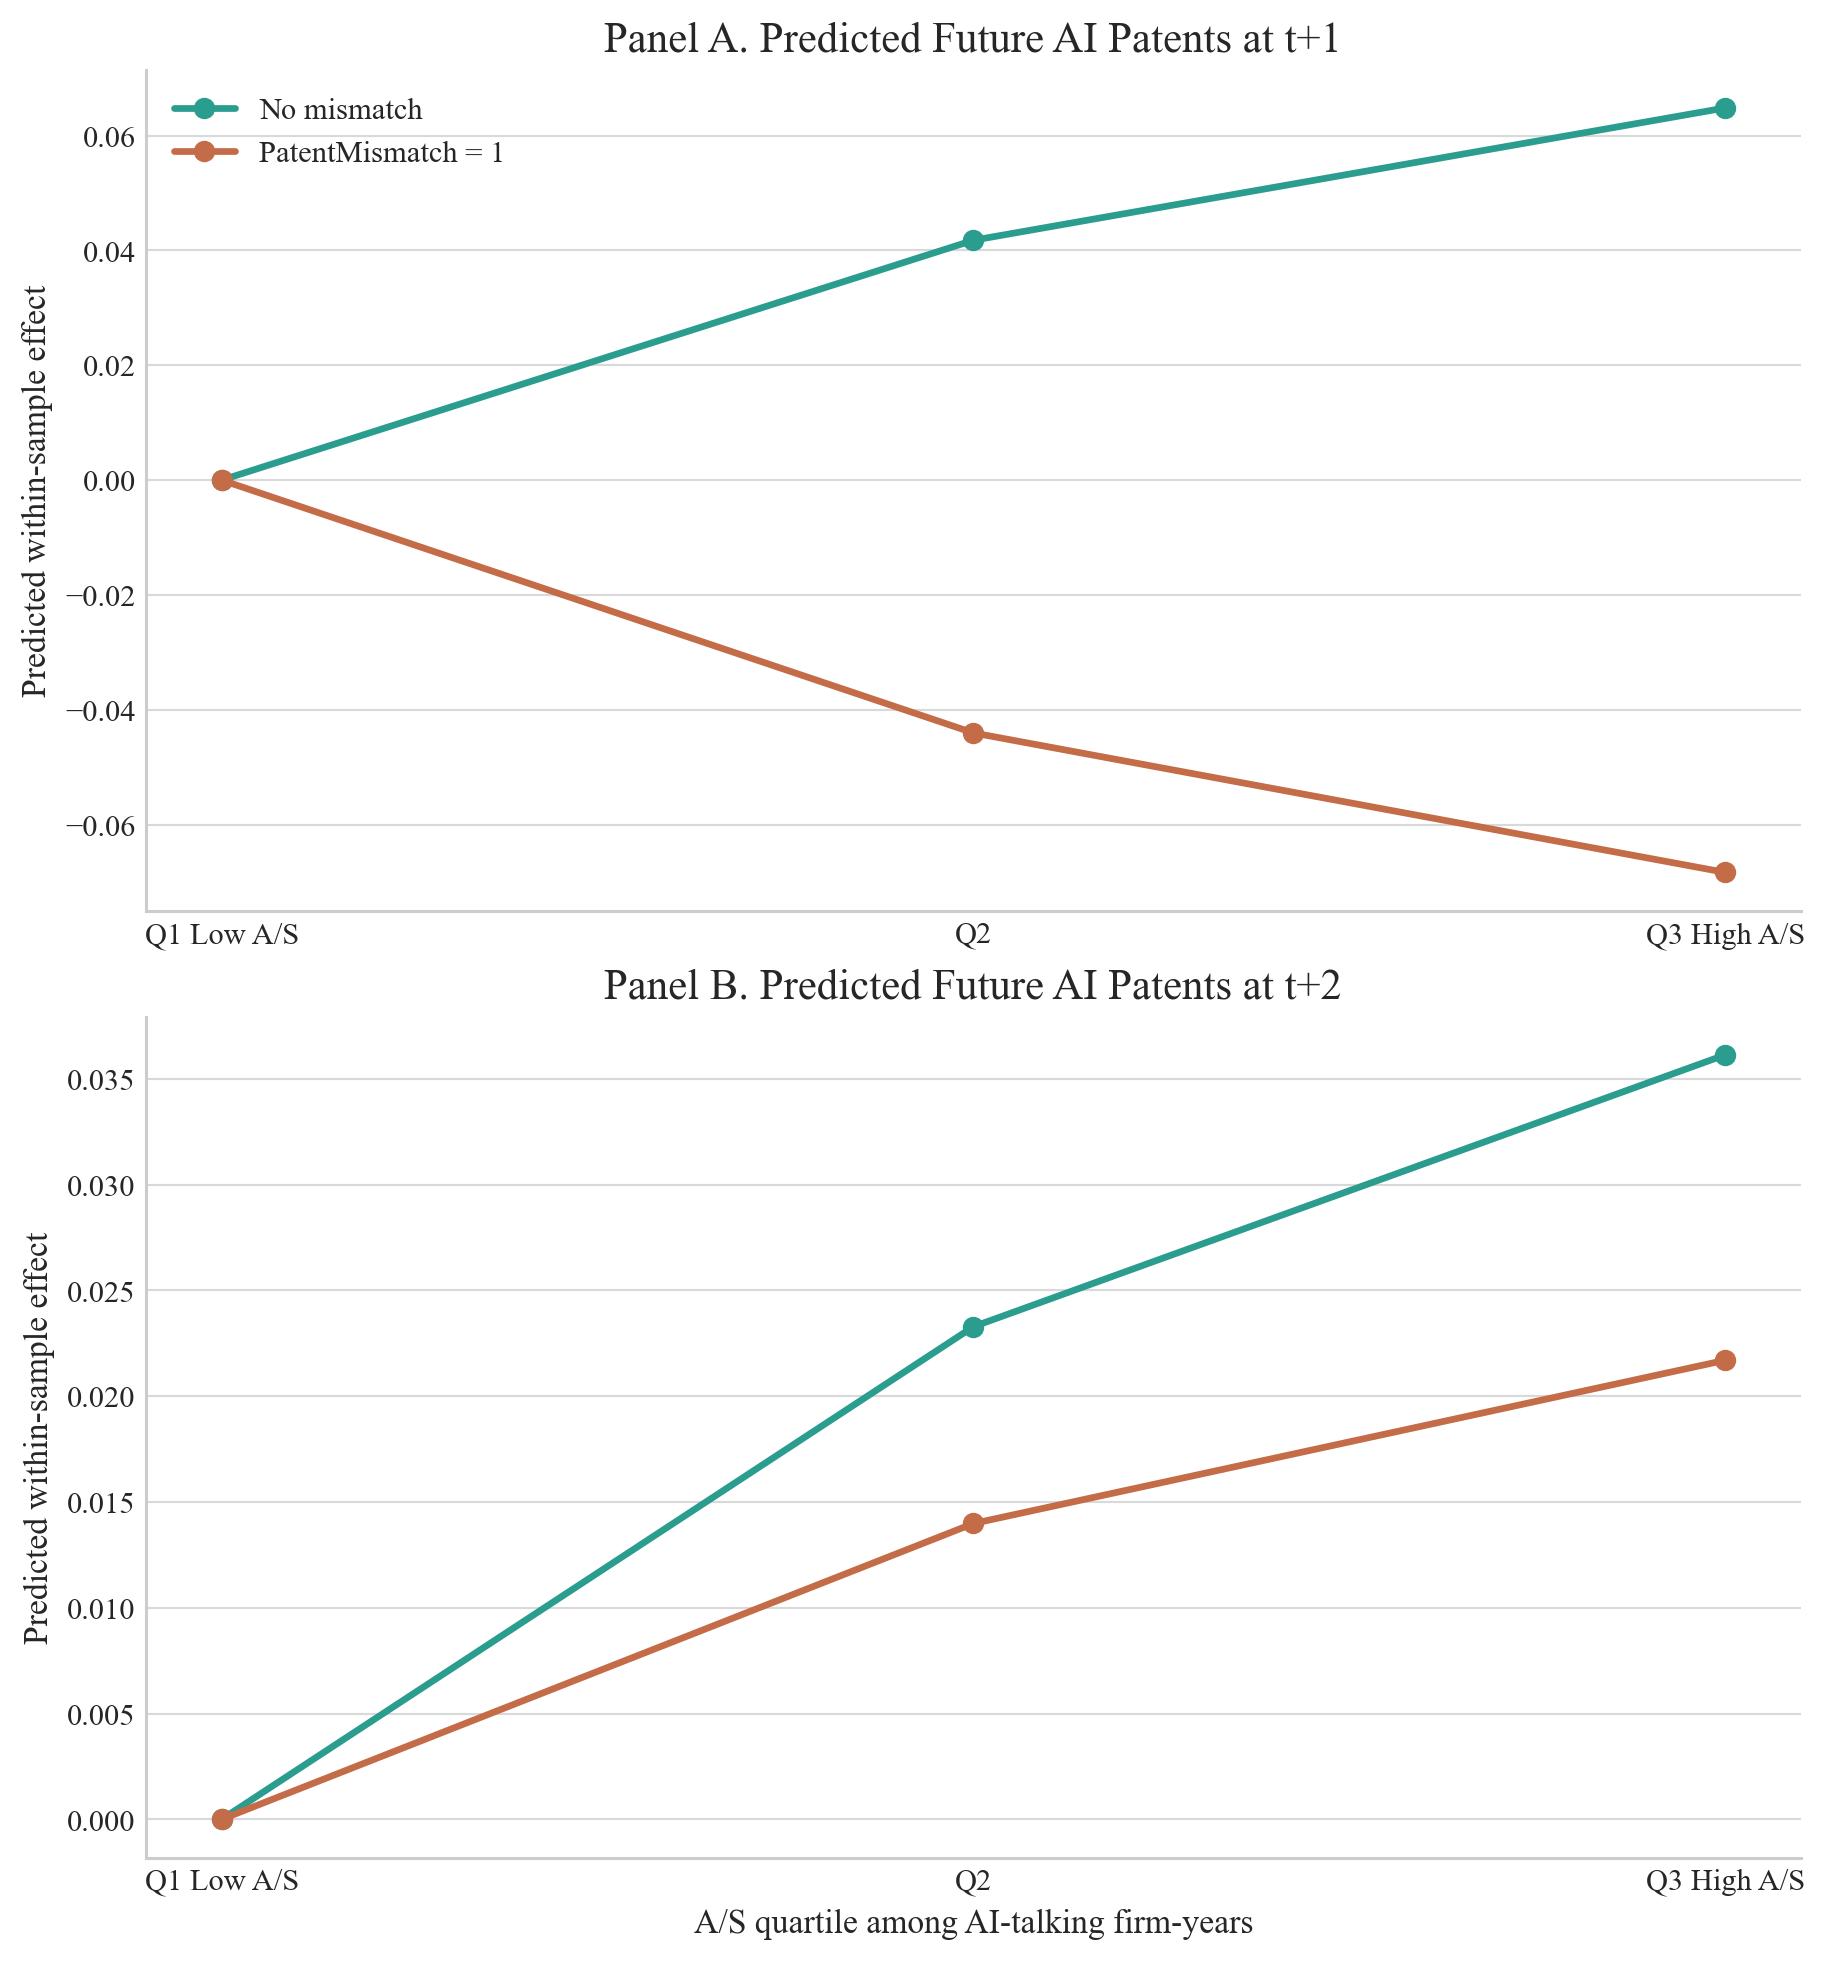
\includegraphics[width=\textwidth]{figures/figure5.png}
\caption{Patent alignment and mismatch by AS-ratio quantile}
\label{fig:mismatch_alignment}
\end{figure}

\subsection{Exploratory evidence around the release of ChatGPT}

The final question is whether the disclosure-credibility patterns intensify after the public release of ChatGPT. Table~\ref{tab:chatgpt_did} reports the baseline post-ChatGPT difference-in-differences specifications, where treated firms are those with weak pre-period AI capability, firms with zero pre-period AI-related patents, and either a low pre-period AS ratio or no pre-period actionable disclosure. The strongest response appears in PatentMismatch: the post-ChatGPT interaction is 0.1745 (p $<$ 0.001). By contrast, the CAR filing-date interaction is 0.0076 (p = 0.307), and the post-filing BHAR interaction is 0.0075 (p = 0.737). In other words, the post-ChatGPT evidence is most consistent with an expansion in low-credibility AI talk rather than with a comparably sharp immediate repricing of that talk by the market.

These results should be interpreted cautiously. The PatentMismatch panel shows a strong post-2022 response, whereas the corresponding CAR panel does not. The pretrend diagnostics are also less comfortable for PatentMismatch than for CAR. For that reason, the post-ChatGPT block is best viewed as exploratory evidence that the late-2022 period amplified the disclosure-credibility tension documented elsewhere in the paper.

\tablepdf
{Exploratory post-ChatGPT difference-in-differences evidence}
{tab:chatgpt_did}
{The table reports exploratory post-ChatGPT difference-in-differences evidence on whether the post-2022 period is associated with a sharper expansion in low-credibility AI disclosure.}
{tables/table8.png}
\FloatBarrier

The appendix collects the supporting material that is useful for interpretation but not essential to the main narrative. Appendix A reports the updated measurement audit and the sample-attrition map. Appendix B reports the broader patent-timing validation tables and the longer-horizon mismatch specification. Appendix C reports the determinants, heterogeneity, and ancillary consequence tests, including the fuller post-ChatGPT event-study figure.